\begin{figure*}[hbtp]
  \centering
  \subfigure[No continued passes]{
    \label{fig:subrefine-stages--01}
    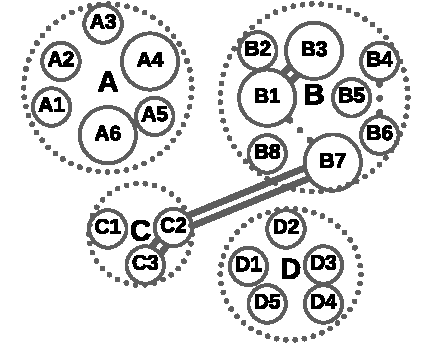
\includegraphics[width=0.31\linewidth]{out/subrefine-stages01.pdf}
  }
  \subfigure[Full Refine]{
    \label{fig:subrefine-stages--02}
    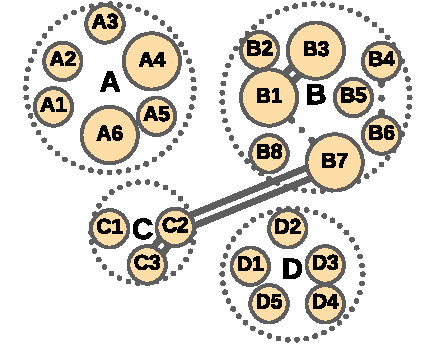
\includegraphics[width=0.31\linewidth]{out/subrefine-stages02.pdf}
  }
  \subfigure[Subset Refine]{
    \label{fig:subrefine-stages--03}
    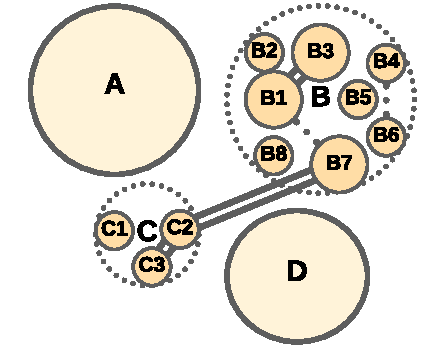
\includegraphics[width=0.31\linewidth]{out/subrefine-stages03.pdf}
  } \\[-1ex]
  \caption{Comparison of \textit{No continued passes}, \textit{Full Refine}, and \textit{Subset Refine} methods. Here, circles represent communities (or subcommunities post refinement), dotted circles denote old parent communities during the local-moving phase\ignore{community bounds}, dotted lines indicate edge deletions, double lines signify edge insertions, and a brown fill indicates mandated further processing. Pre-existing edges are not shown\ignore{for simplicity}. With \textit{No continued passes}, all communities are refined after the local-moving phase; however, it may converge prematurely with small batch updates, resulting in suboptimal community structures. The \textit{Full Refine} method processes all refined communities after they are aggregated into super-vertices. In contrast, with the \textit{Subset Refine} method, we selectively refine only a subset of communities based on the batch update, leaving the remaining communities unchanged.}
  \label{fig:subrefine-stages}
\end{figure*}
